\section{Répartition des tâches}

Dans le but de pouvoir travailler séparément et de manière autonome sur chaque module lors de l'implémentation, nous avons rigoureusement travaillé les spécifications techniques et l'architecture globale de l'application. Les tâches de développement ont ensuite été  menées de manière parallèle par chacun des membres de l'équipe :

\begin{itemize}
\item Namrata était résponsable du module d'analyse,
\item Clément du raisonnement,
\item Thibaut de la mémoire,
\item et William de l'architecture client-serveur et des jeux.
\end{itemize}   

Nous nous sommes réunis tout au long du développement pour assurer l'avancement global du projet et répondre aux interrogations de chacun.

\section{Outils utilisés}

\subsection{Gestionnaire de versions}
Tout au long du projet, nous avons utilisé \emph{git} : un gestionnaire de version décentralisé. Un tel outil permet la mise en commun des travaux, la gestion des versions et la gestion des \emph{merges}\footnote{Fusion de deux fichiers différents.}. 

\begin{center}
	
\includegraphics[width=0.3\textwidth]{files/outils/git}	
\end{center}

Nous avons choisi \emph{git} pour plusieurs raisons :

\begin{itemize}
\item plutôt simple d'utilisation (par rapport à ses homologues comme \emph{SVN}),
\item hébergement gratuit via GitHub (sous condition de diffusion du code sous une licence libre),
\item \emph{git} est une solution libre sous licence \gls{GPLv2}.
\end{itemize}

\subsection{EtherPad, un éditeur de texte collaboratif}
\emph{EtherPad} se présente sous la forme d'un éditeur de texte léger permettant de faire un minimum de mise en page.

\begin{figure}[H]
	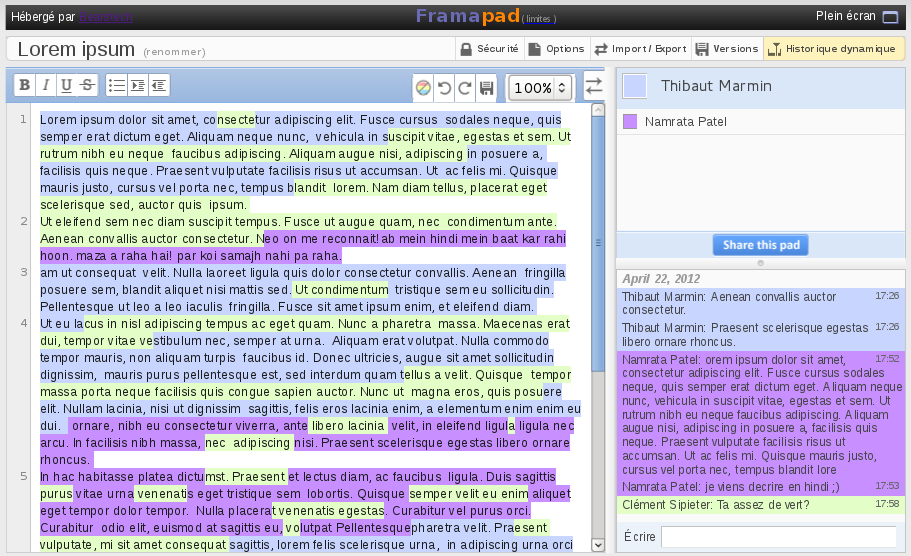
\includegraphics[width=\textwidth]{files/outils/etherpad_screenshot}	
	\caption{Aperçu de l'interface d'\emph{EtherPad} hébergé sur \emph{framapad} (site mis à disposition par Framasoft utilisant le code d'EtherPad).}
	\label{etherpad_screenshot}
\end{figure}

\begin{center}
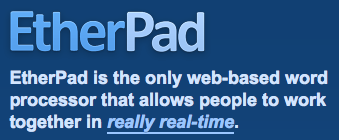
\includegraphics[width=0.4\textwidth]{files/outils/etherpad}
\end{center}

L'interface d'\emph{EtherPad} se présente sous la forme d'une interface web (figure \ref{etherpad_screenshot}) où chaque utilisateur connecté possède une couleur. La singularité de cet outil réside dans le fait que toutes les modifications effectuées sur le pad sont visibles par tous en temps réel.

Un chat est également disponible ce qui facilite la collaboration entre les utilisateurs connectés.

Il est important de noter qu'\emph{EtherPad} est sous licence \gls{Apache v2}.

\subsection{Visualisation de graphes}

Pour débugger la base de données Neo4j, nous avons utilisé \emph{Gephi}, un utilitaire basé sur la \emph{NetBeans Platform}.

\begin{center}

\includegraphics[width=0.4\textwidth]{files/outils/gephi}
\end{center}

Il permet de visualiser et de manipuler des graphes. C'est un outil libre qui embarque quelques plugins dont un connecteur Neo4j permettant l'import de bases de données du SGBD.

\subsection{Outils de développement}
Voici une liste non exhaustive des outils que nous avons utilisés lors de nos développements :
\begin{description}
\item[Eclipse / NetBeans] Il s'agit des deux principaux EDI\footnote{Environnement de Développement Intégré} libres, permettant une vérification et compilation dynamique du code écrite.
\item[Javadoc] Nous avons pris soin de documenter la totalité de notre code dans le but de rentre notre code réutilisable. Javadoc est aujourd'hui devenu un standard industriel utilisé par la majorité des développement Java.
\item[Log4j] Librairie Java libre qui permet la journalisation sous formes variées (stdout\footnote{Flux de sortie standard.}, fichiers de log, envoie de mail, etc.).
\item[YourKit Java Profiler] Afin de permettre d'optimiser certaines méthodes, nous avons utilisé cet outil en version d'évaluation (sous licence propriétaire). Il s'intègre parfaitement dans la plupart des environnement de développement.
\end{description}